%!TEX root = ../main.tex

\section{Tree-Like Unraveling}\label{sec:unraveling}
We next describe a notion of \emph{tree unravellings} for $\FGF$.
A truncated form of these unravellings will be employed afterwards in the construction of the companion structures required in~\cref{thm:main-technical-thm}.
The truncation is necessary because the tree unraveling must sometimes be infinite even for finite structures, since it is an acyclic structure.\bbebox{Don't like it. Rewrite. How about: As tree unravellings of structures containing cycles are infinite, the truncation is necessary here.}
This is similar to the approach taken by Otto to construct the finite companions for the van Benthem charactisation of modal logic with universal modalities~\cite[Proof of Lemma 38]{Otto04}.

Let $\str{A}$ be a structure with an associated binary relation $\relNext^{\str{A}}$.
For a pair $(\eleme_1, \eleme_2) \in \relNext^{\str{A}}$, we call the element $\eleme_2$ a \emph{child} of $\eleme_1$. Respectively, we call $\eleme_1$ a \emph{parent} of $\eleme_2$.
A \emph{root} is an element without parents.
The set of $\emph{descendants}$ of an element $\eleme$ is the smallest set containing $\eleme$ that is closed under taking children (\ie{} if an element is in the set then so are its children).
We call a structure $\str{A}$ a \emph{forest} if $\relNext^{\str{A}}$ every element has at most one parent and is a descendant of some root.\bbeside{Better :)}
A model is a tree model if it is a forest and has exactly one root.
It is well-known that with a suitable notion of unravelling~\cite[Prop. 3]{Rosen97}\bbeside{Always use tilde before cite.} one can show that every satisfiable modal logic formula has a tree model.

Our goal is to have an unravelling for $\FGF$ satisfying the following theorem:
\begin{theorem}\label{thm:inf-unraveling-upgrading}
  Let $\str{A}, \elemtuplea \bisimto_{\FGF} \str{B}, \elemtupleb$ for two pointed $\sigma$-structures.
  Then there are tree models $\unravel{A}, \elemtuptuplea$ and $\unravel{B}, \elemtuptupleb$ which are both:
  \begin{itemize}
    \item $\FGF$-similar to the original structures: $\unravel{A}, \elemtuptuplea \bisimto_{\FGF} \str{A}, \elemtuplea$ and $\unravel{B}, \elemtuptupleb \bisimto_{\FGF} \str{B}, \elemtupleb$
    \item $\GF$-bisimilar: $\unravel{A}, \elemtuptuplea \bisimto_{\GF} \unravel{B}, \elemtuptupleb$
  \end{itemize}
\end{theorem}
The \emph{HAF}-unravelling~\cite[Sec 3.3]{Bednarczyk21}\bbeside{It would be nice to introduce HAFs. Otherwise it is hard to verify your claims. Moreover, it would be nice for the thesis to have the comparison.} introduced by Bednarczyk for $\FGF$ yields a tree model, but unfortunately fails the above theorem.
Consider the two finite structures shown in \cref{fig:unravel-haf}, which are both identical to their HAF-unravelling as they are already HAFs.
Yet, they can be distinguished by the $\GF$ sentence $\forall{x,y}. \relE(x,y) \to \exists a. \relP(x,y,z)$.\bbeside{Should a be z?}
Since both structures are $\FGF$ bisimilar, this shows that HAF-unravellings do not satisfy \ref{thm:inf-unraveling-upgrading}\bbeside{cref not ref} even in the finite case.
\begin{figure}
  \centering
    \begin{tikzpicture}[baseline=(current bounding box.north)]
        \draw[tolbrightGreen, line cap=round, line width=2em] (-0em,8em) -- ++(0,-8em);
        \draw[tolbrightYellow, line cap=round, line width=0.5em, -{Latex[length=2em]}] (0,4em) -- (0,0em);

        \draw [black, line width=0.1em, fill=white] (0em, 8em) circle [radius=0.8em] node[anchor=center] {1};
        \draw [black, line width=0.1em, fill=white] (0em, 4em) circle [radius=0.8em] node[anchor=center] {2};
        \draw [black, line width=0.1em, fill=white] (0em, 0em) circle [radius=0.8em] node[anchor=center] {3};

        \begin{scope}[xshift=10em]
            \draw[tolbrightGreen, line cap=round, line width=2em] (-0em,8em) -- ++(0,-8em);
            \draw[tolbrightYellow, line cap=round, line width=0.5em, -{Latex[length=2em]}] (0em,4em) -> (6em,2em);
            \draw[tolbrightYellow, line cap=round, line width=0.5em, -{Latex[length=2em]}] (0,4em) -- (0,0em);

            \draw [black, line width=0.1em, fill=white] (0em, 8em) circle [radius=0.8em] node[anchor=center] {1};
            \draw [black, line width=0.1em, fill=white] (0em, 4em) circle [radius=0.8em] node[anchor=center] {2};
            \draw [black, line width=0.1em, fill=white] (0em, 0em) circle [radius=0.8em] node[anchor=center] {3};
            \draw [black, line width=0.1em, fill=white] (6em, 2em) circle [radius=0.8em] node[anchor=center] {3'};

            \node[tolbrightGreen] at (-2em, 6em) {P};
            \node[tolbrightYellow] at (-1.5em, 2em) {E};
            \node[tolbrightYellow] at (3em, 4em) {E};
        \end{scope}

        \node[font=\Large] at (5em, 4em) {$\sim_{FGF}$};

        \node[tolbrightGreen] at (-2em, 6em) {P};
        \node[tolbrightYellow] at (-1.5em, 2em) {E};
    \end{tikzpicture}%
    \caption{Two FGF-bisimilar HAFs which are not GF-bisimilar. Relations are drawn top to bottom, so the green area marks the relation $\relP(1,2,3)$}%
    \label{fig:unravel-haf}
\end{figure}

For our new\bbeside{notion of?} \FGF-unravelling, we make use of the equivalence between bisimulation\bbeside{s?} and games~\cite[Sec. 1.2.1]{Gradel014}.
The $\FGF$-\emph{bisimulation game} is played on two structures $\str{A}$ and $\str{B}$ by two players, Spoiler and Duplicator.
We initialize the game by selecting a live tuple from each structure, $\elemtuplea$ and $\elemtupleb$.
In each turn, Spoiler first chooses a structure.
The game is symmetric, so let us assume that spoiler chooses the structure $\str{A}$.
Spoiler then selects an infix $\elemtupleafromto{i}{j}$ of the currently selected tuple and a new live tuple $\elemtuplec$ which has $\elemtupleafromto{i}{j}$ as a prefix.
We use the terms \emph{shared elements} for the prefix $\elemtuplecfromto{1}{j-i+1}$ and \emph{unshared elements} for the remaining elements $\elemtuplecfromto{j-i+1+1}{|\elemtuplec|}$.
Duplicator must then find a live tuple $\elemtupled$ in $\str{B}$ which has $\elemtuplebfromto{i}{j}$ as a prefix.
\bbeside{Important! It looks like that you missed the fact that types of freshly created tuples should be the same.}
Note that some of the unshared elements may still be elements from $\elemtuplea$, but Duplicator is not required to preserve equivalences between the unshared elements and elements from $\elemtuplea$, while Duplicator must preserve the shared prefix.
The game then continues with the next turn, with $\elemtuplec$ and $\elemtupled$ as the new selected tuples.
Spoiler wins the game if Duplicator is unable to find matching elements.
The possible actions of Spoiler are equivalent to the back-and-forth conditions for $\FGF$-bisimulation.
A winning strategy for Duplicator is thus equivalent to a $\FGF$-bisimulation between the two structures, and vice-versa.
We next describe the domain of the unravelling, which is based on a sequence of actions in this game.

\bbebox{It would be nice to add some lemma here, e.g. that duplicator has a winning strategy if and only if there is a bisimulation between... I know that you said this, but it makes sense to make it more explicit. I also think that a good idea would be to introduce $\ell$-round games, as we will use them afterwards.}

\noindent \textbf{Domain of the unraveling}
Let $\str{A}, \elemtuplea^{(0)}$ be a pointed $\sigma$-structure.
We define a bisimulation sequence as the sequence of actions that Spoiler may take in a $\FGF$-bisimulation game involving this structure.
Formally, a \emph{bisimulation sequence} of length $\ell$ is a sequence of the form $\elemtuplea^{(0)}(i^{(1)}, j^{(1)})\elemtuplea^{(1)}\cdots(i^{(\ell)}, j^{(\ell)})\elemtuplea^{(\ell)}$, where each $a^{(k)}$ is a live tuple in $\str{A}$ and $i^{(k)}, j^{(k)}$ are indices such that $\elemtupleafromto{i^{(k)}}{j^{(k)}}^{(k-1)} = \elemtupleafromto{1}{j^{(k)}-i^{(k)}+1}^{k}$.
The set $\Seq{A}$ of all bisimulation sequences for a structure $\str{A}$ collects all possible ways in which Spoiler can explore this structure.
For any length $\ell$ bisimulation sequence, if $\str{B}, \elemtupleb^{(0)}$ is a $\sigma$-structure that is \FGF-bisimilar to $\str{A}, \elemtuplea^{(0)}$, then we can apply \ref{bisim:fforth} $\ell$ times to find tuples $\elemtupleb^{1}, \ldots, \elemtupleb^{\ell}$ for a corresponding bisimulation sequence in $\str{B}$.
These represent the actions of Duplicator in the game.
Below are some examples of bisimulation sequences:
\begin{figure}[H]
  \centering
    \begin{minipage}[t]{0.2\textwidth}
        \raggedleft
        \vspace{0pt}
        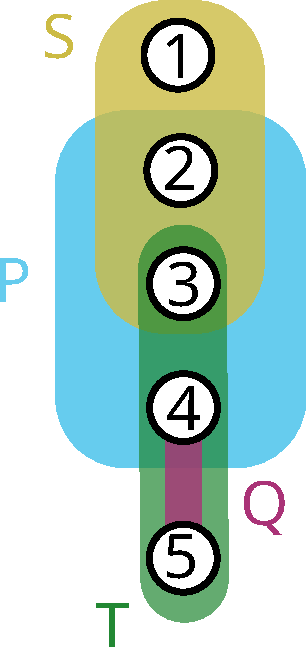
\includegraphics[scale=0.5]{res/example-struct-1}
    \end{minipage}
    \hspace{4em}
    \begin{minipage}[t]{0.6\textwidth}
      {%
      \newcommand{\tups}{{\color{tolbrightYellowDarker}\elemtuples}}%
      \newcommand{\tupp}{{\color{tolbrightCyanDarker}\elemtuplep}}%
      \newcommand{\tupt}{{\color{tolbrightGreen}\elemtuplet}}%
      \newcommand{\tupq}{{\color{tolbrightPurple}\elemtupleq}}%
      The picture on the left shows a structure with the relations: $(1,2,3) \in \relS^{\str{A}}$, $(2,3,4) \in \relP^{\str{A}}$, $(3,4,5) \in \relT^{\str{A}}$, $(4,5) \in \relQ^{\str{A}}$

      \vspace{1ex}
      Let $\tups = (1, 2, 3), \tupp = (2, 3, 4), \tupt = (3, 4, 5), \tupq = (4,5)$.

      \vspace{1ex}
      Some examples of bisimulation sequences in this structure are:
      \begin{itemize}
          \item $\tups(3,3)\tupt$
          \item $\tups(2,3)\tupp(2,3)\tupt$
      \end{itemize}

      Bisimulation sequences are not required to use maximal infixes, so the following are also valid bisimulation sequences:
      \begin{itemize}
          \item $\tups(2,2)\tupp$
          \item $\tups(3,3)\tupt(2,2)\tupq$
      \end{itemize}
      }
    \end{minipage}
    \caption{Examples for bisimulation sequences}
\end{figure}

Consider the last tuple of a bisimulation sequence.
This tuple has a prefix of elements which are shared with the previous tuple, and a suffix of unshared elements, as in the \FGF-bisimulation game.
We now introduce a counter to distinguish these unshared elements.
The \emph{unraveling domain} $\unraveldom{A} \subseteq \Seq{A} \times \mathbb{N}$ for $\str{A}$ is a set, with $(\sigma, k) \in \unraveldom{A}$ if:
\begin{itemize}
  \item $\sigma = \elemtuplea$, then $k \ge 1$ and $k \le |\elemtuplea|$, or
  \item $\sigma = \cdots (i,j) \elemtuplea$, then $k \ge (j-i+1) + 1$ and $k \le |\elemtuplea|$
\end{itemize}
For an element $e \in \unraveldom{A}$ where $e = (\rho, k)$, we use the notation $\seq{e} = \rho$ and $\ctr{e} = k$ to denote the sequence and the counter of this element, respectively.
Let $\elemtuplea$ be the last tuple of $\seq{e}$, so $\seq{e} = \cdots \elemtuplea$.
Since the counter is an index into last tuple, we can define the projection $\pi(e)$ as: $\pi(e) = \elema_{\ctr{e}}$.
On the unraveling domain, the binary relation $\relNext \subseteq \unraveldom{A} \times \unraveldom{A}$ is defined such that $(s, t) \in \relNext$ if either:
\begin{description}
  \item[\desclabel{(addCtr)}{next:addctr}] $\seq{s} = \seq{t}$, $\ctr{t} = \ctr{s} + 1$, or
  \item[\desclabel{(addSeq)}{next:addseq}] $\seq{t} = \seq{s} (i,j) \elemtuplea$ for some $i, j, \elemtuplea$ and $\ctr{s} = j, \ctr{t} = (j - i + 1) + 1$
\end{description}
The unraveling domain with the $\relNext$ relation is a forest.
The roots are elements with counters equal to one and sequences of length one.
Every other element has a unique parent: for elements with counters not equal to $(j - i + 1) + 1$ (where $i$ and $j$ are the indices for the last action in the sequence), the only element that links to this element is the element with the counter decreased by one.
For elements with counter equal to $(j - i + 1) + 1$, the element with counter decreased by one is not part of the unraveling domain.
Therefore, the only element linking to this element is the one where the last action is removed from the sequence, by the~\ref{next:addseq} case of the definition.
As the parent in each case has either a shorter sequence or a lower counter and a sequence of the same length, taking parents repeatedly must end in a root at some point.
So every element is a descendant of some root and has at most one parent, as wanted.

The definition of $\relNext$ has the following nice property: if $(s,t) \in \relNext$ and $t$ projects to $a_{k}$ for $k > 1$, then $s$ projects to $a_{k-1}$, where $k = \ctr{t}$ and $\elemtuplea$ is the tuple such that $\seq{t} = \cdots \elemtuplea$.
We prove this by case analysis on the two cases of $\relNext$.
The~\ref{next:addctr} case is simple: in this case $\seq{s} = \seq{t}$ and $\ctr{s} = k - 1$, so the property follows directly from the definition of $\pi$.
For the~\ref{next:addseq} case, let $\seq{t} = \seq{s} (i,j) \elemtuplea$ and $\seq{s} = \cdots \elemtupleb$.
Further, in this case $k = (j - i + 1) + 1$ and $\ctr{s} = j$.
By the fact that $\seq{t}$ is a bisimulation sequence, we know that $\elemtupleafromto{1}{j-i+1} = \elemtuplebfromto{i}{j}$.
In particular, it follows that $\pi(s) = b_{j} = a_{j-i+1} = a_{k-1}$, concluding the proof.

\noindent
\textbf{Relations in the unraveling}
A tuple of elements $(e_{1}, \ldots, e_{n})$ is a \emph{next chain} if adjacent elements are related by $\relNext$, so $(e_{i}, e_{i+1}) \in \relNext$ for all $i$.
If the length $n$ of the next chain is less than $\ctr{e_{n}}$, then we know by the previous observation that the projection of the chain is $\elemtuplee_{(\ctr{e_{n}}-n+1)\ldots{}\ctr{e_{n}}}$, where $\elemtuples$ is the last tuple of $\seq{e_{n}}$.
We define the tree unraveling such that relations are only realized by tuples which are next chains.
Additionally, we limit the length of the chain to be less than the counter of the last element of the tuple.
For this, let $\mathtt{bound}(\elemtuptupler)$ of some tuple $\elemtuptupler$ be equal to $\ctr{\elemtuptupler_{|\elemtuptupler|}}$ (the counter of the last element of the tuple).
Let $\str{A}, \elemtuplea$ be a $\sigma$-structure and $\unraveldom{A}$ be the unraveling domain.
Let $\elemtuptuplea = ((\elemtuplea, 1), \ldots, (\elemtuplea, |\elemtuplea|))$.
The \emph{tree unraveling} $\unravel{A}, \elemtuptuplea$ is the tree with root $(\elemtuplea, 1)$ and all descendants according to the relation $\relNext$.
For relations $\relR \in \sigma$, we let $\elemtuptupler \in \relR^{\unravel{A}}$ if and only if:
\begin{enumerate}
  \item $\pi[\elemtuptupler] \in \relR^{}$,
  \item $\bigwedge_{k=1}^{|\elemtuptupler|-1}{(\elemr_{k},\elemr_{k+1}) \in \relNext}$, and
  \item $|\elemtuptupler| \le \mathtt{bound}(\elemtuptupler)$
\end{enumerate}
The second and third condition restrict live tuples to be next chains with a length bounded by the counter of the last element of the tuple, as discussed before.

We illustrate the construction with an example.
Recall the left structure from \cref{fig:unravel-haf}.
Let $\elemtuplep = (1,2,3)$ and $\elemtuplee = (2,3)$.
The picture below shows the tree unraveling with root $(\elemtuplep, 1)$.
\begin{figure}[H]
  \centering
  \begin{tikzpicture}
    \draw[tolbrightGreen, line cap=round, line width=2.2em] (-0em,8em) -- ++(0,-8em);
    \draw[tolbrightYellow, line cap=round, line width=0.5em, -{Latex[length=2em]}] (0em,4em) -> (6em,1em);
    \draw[tolbrightYellow, line cap=round, line width=0.5em, -{Latex[length=2em]}] (0,4em) -- (0,0em);

    \draw [black, line width=0.1em, fill=white] (0em, 8em) ellipse (1em and 0.8em) node[anchor=center] {$(\elemtuplep, 1)$};
    \draw [black, line width=0.1em, fill=white] (0em, 4em) ellipse (1em and 0.8em) node[anchor=center] {$(\elemtuplep, 2)$};
    \draw [black, line width=0.1em, fill=white] (0em, 0em) ellipse (1em and 0.8em) node[anchor=center] {$(\elemtuplep, 3)$};
    \draw [black, line width=0.1em, fill=white] (6em, 0em) ellipse (3em and 1em) node[anchor=center] {$(\elemtuplep(2,2)\elemtuplee, 2)$};

    \node[tolbrightGreen] at (-2em, 6em) {P};
    \node[tolbrightYellow] at (-1.5em, 2em) {E};
    \node[tolbrightYellow] at (3em, 4em) {E};
  \end{tikzpicture}
\end{figure}
First, observe that the structure is isomorphic to the structure on the right in \cref{fig:unravel-haf}.
It is easy to see that the structure on the right also unravels to an isomorphic structure with this construction.
Thus, at least in this example, \cref{thm:inf-unraveling-upgrading} is not violated.
Consider the tuples $\elemtuptuplea = ((\elemtuplep, 1), (\elemtuplep, 2), (\elemtuplep, 3))$ and $\elemtuptupleb = ((\elemtuplep, 1), (\elemtuplep, 2), (\elemtuplep(2,2)\elemtuplee, 2))$.
These tuples have equal projections: $\pi(\elemtuptuplea) = \pi(\elemtuptupleb) = \elemtuplep$.
But $\elemtuptuplea \in \relP^{\unravel{A}}$ while $\elemtuptupleb \notin \relP^{\unravel{A}}$.
This is because $\mathtt{bound}(\elemtuptupleb) = 2$ and $|\elemtuptupleb| = 3$, so the bound for $\elemtuptupleb$ is not large enough.

We now prove \cref{thm:inf-unraveling-upgrading} for this unraveling.
\begin{proof}
  \bfbox{write proof}
\end{proof}
